\begin{frame}{Finding the Best Line}
    We want a line with small residuals, so it might make sense to try to minimize 
    \[
        \sum_{i=1}^n e_i = \sum_{i=1}^n (y_i - \hat{y}_i)
    \]
    ...but this will give us very large negative residuals!
\end{frame}

\begin{frame}{Finding the Best Line}
    As with the standard deviation, we will use squares to shift the focus to magnitude:
    \[
        \sum_{i=1}^n e_i^2 = \sum_{i=1}^n (y_i - \hat{y}_i)^2
    \]
\end{frame}

\begin{frame}{Finding the Best Line}
    \begin{align*}
        \sum_{i=1}^n e_i^2 &= \sum_{i=1}^n (y_i - \hat{y}_i)^2 \\
                &= \sum_{i=1}^n [y_i - (b_0 + b_1 x_i)]^2
    \end{align*}
    The values of $b$ that minimize this will make up our regression line.
    
    \vspace{1cm}This is called the \textbf{Least Squares Criterion}.
\end{frame}

\begin{frame}{Finding the Best Line}
    To fit a \textbf{least squares regression}, we require
    \begin{itemize}
        \item Linearity. The data should show a linear trend.
        \item Nearly normal residuals. The residuals should be well-approximated by a normal distribution.
        \item Constant variability. As we move along $x$, the variability around the regression line should stay constant.
        \item Independent observations. This will apply to random samples.
    \end{itemize}
\end{frame}

\begin{frame}{Finding the Least Squares Line}
    We want to estimate $\beta_0$ and $\beta_1$ in the equation
    \[
        y = \beta_0 + \beta_1 x + \epsilon
    \]
    by minimizing $\sum_{i=1}^n (y_i - \hat{y}_i)^2$.
\end{frame}

\begin{frame}{Finding the Least Squares Line}
    This turns out to be remarkably straightforward! The slope can be estimated as
    \[
        b_1 = \frac{s_y}{s_x}R
    \]
    and the intercept by 
    \[
        b_0 = \bar{y} - b_1 \bar{x}
    \]
\end{frame}

\begin{frame}{Example}
    The \texttt{faithful} dataset in \texttt{R} has two measurements taken for the Old Faithful Geyser in Yellowstone National Park:
    \begin{itemize}
        \item \texttt{eruptions}: the length of each eruption
        \item \texttt{waiting}: the time between eruptions
    \end{itemize}
    Each is measured in minutes.
\end{frame}

\begin{frame}{Example}
    \begin{center}
        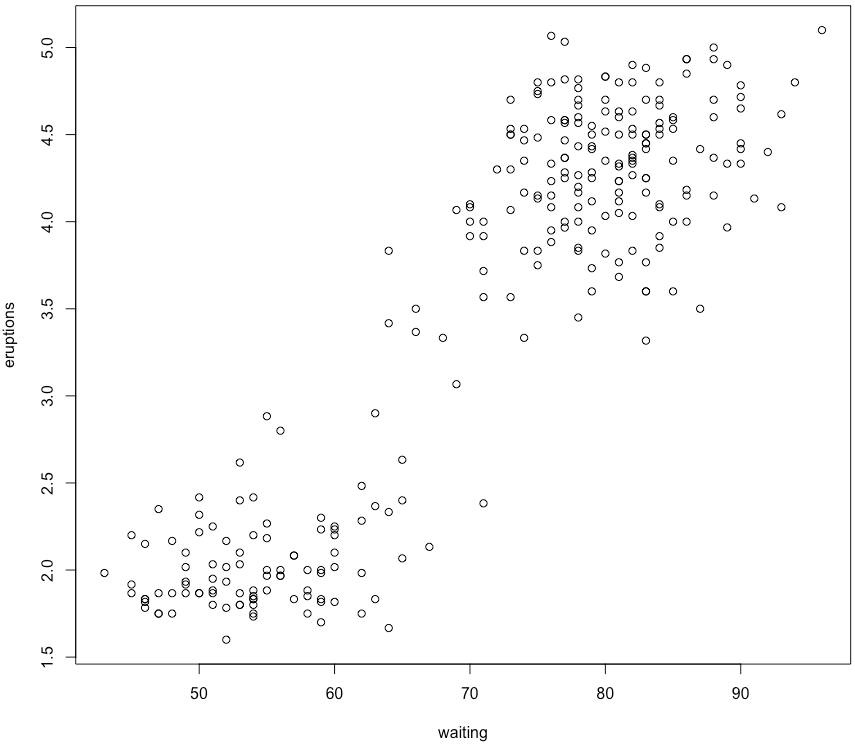
\includegraphics[scale=0.25]{images/geyserscatter.png}
    \end{center}
    
    \vspace{-0.5cm}We want to see if we can use the wait time to \textit{predict} eruption duration.
\end{frame}

\begin{frame}{Example}
    The sample statistics for these data are
    \begin{table}[]
        \centering
        \begin{tabular}{l cc}
            \hline
             & \texttt{waiting} & \texttt{eruptions} \\ \hline
            mean & $\bar{x}=70.90$ & $\bar{y}=3.49$ \\
            sd & $s_x=13.60$ & $s_y=1.14$ \\ \hline
            && $R = 0.90$ \\ \hline
        \end{tabular}
    \end{table}
    Find the linear regression line and interpret the parameter estimates.
\end{frame}

\begin{frame}{Example}
    \begin{center}
        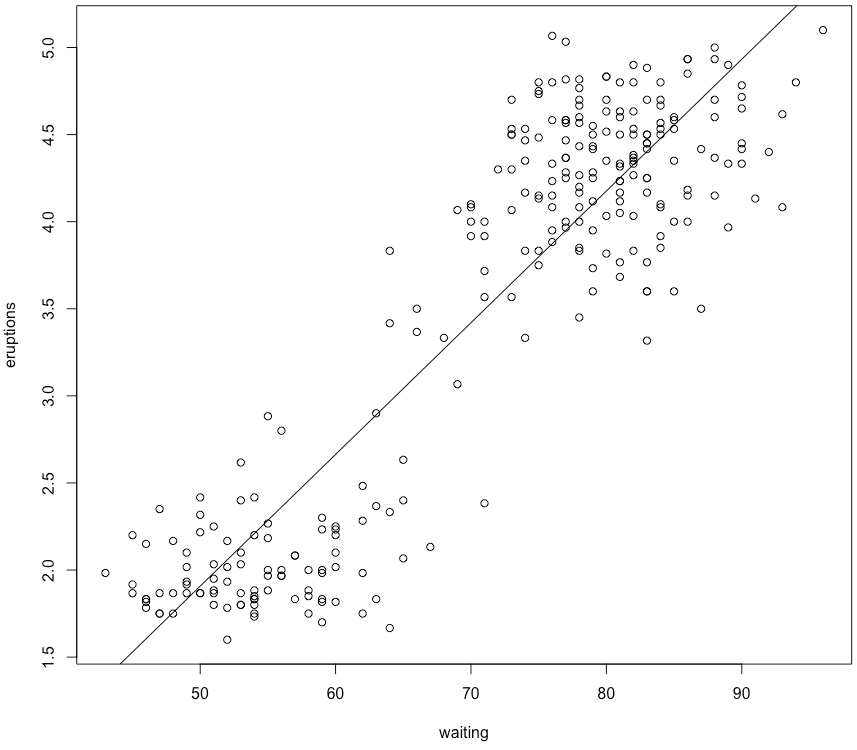
\includegraphics[scale=0.25]{images/geysreg.png}
    \end{center}
\end{frame}

\begin{frame}{Hypothesis Testing in Linear Regression}
    Whenever we estimate a parameter, we want to use a hypothesis test to think about our confidence in that estimate.
    \begin{itemize}
        \item For $\beta_i$ ($i = 0,1$)
        \begin{align*}
            H_0: \quad \beta_i = 0 \\
            H_A: \quad \beta_i \ne 0 \\
        \end{align*}
        \item We will do this using a one-sample t-test.
    \end{itemize}
\end{frame}

\begin{frame}{Example}
    If we use \texttt{R} to get the coefficients for our \texttt{faithful} data, we get
    \begin{table}[h]
        \centering
        \begin{tabular}{l cccc}
             & Estimate & Std. Error & $t$ value & Pr($>|t|$) \\
            (Intercept) & -1.874016 &  0.160143 & -11.70 &  $<$2e-16 \\
            waiting     & 0.075628  & 0.002219 &  34.09  & $<$2e-16
        \end{tabular}
    \end{table}
    What does this tell us about our parameters?
\end{frame}

\begin{frame}{Extrapolation}
    \begin{itemize}
        \item When we make predictions, we simply plug in values of $x$ to estimate values of $y$. 
        \item However, this has limitations!
        \item We don't know how the data outside of our limited window will behave.
    \end{itemize}
\end{frame}

\begin{frame}{Extrapolation}
    Applying a model estimate for values outside of the data's range for $x$ is called \textbf{extrapolation}.
    \begin{itemize}
        \item The linear model is only an approximation.
        \item We don't know anything about the relationship outside of the scope of our data.
        \item Extrapolation assumes that the linear relationship holds in places where it has not been analyzed.
    \end{itemize}
\end{frame}

\begin{frame}{Extrapolation}
    \begin{center}
        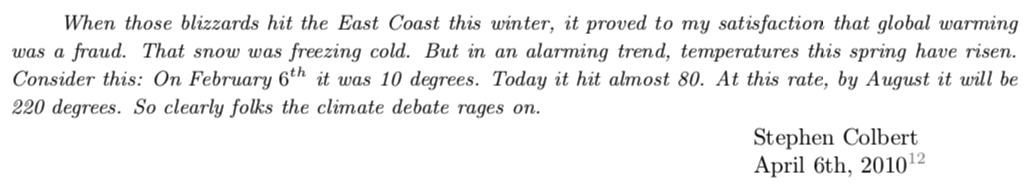
\includegraphics[width=4.75in]{images/colbert.png}
    \end{center}
\end{frame}

\begin{frame}{Example}
    \begin{itemize}
        \item In this data, waiting times range from 43 minutes to 96 minutes. 
        \item Let's predict
        \begin{itemize}
            \item eruption time for a 50 minute wait.
            \item eruption time for a 10 minute wait.
        \end{itemize}
    \end{itemize}
\end{frame}

\begin{frame}{Using $R^2$ to Describe Strength of Fit}
    We've evaluated the strength of a linear relationship between two variables using the correlation coefficient $R$.
    
    \vspace{12pt}However, it is also common to use $R^2$. This helps describe how closely the data cluster around a linear fit.
\end{frame}

\begin{frame}{Using $R^2$ to Describe Strength of Fit}
    Suppose $R^2 = 0.62$ for a linear model. Then we would say
    \begin{itemize}
        \item About 62\% of the data's variability is accounted for using the linear model. 
    \end{itemize}
    And yes, $R^2$ is the square of the correlation coefficient $R$!
\end{frame}

\begin{frame}{Example}
    \begin{center}
        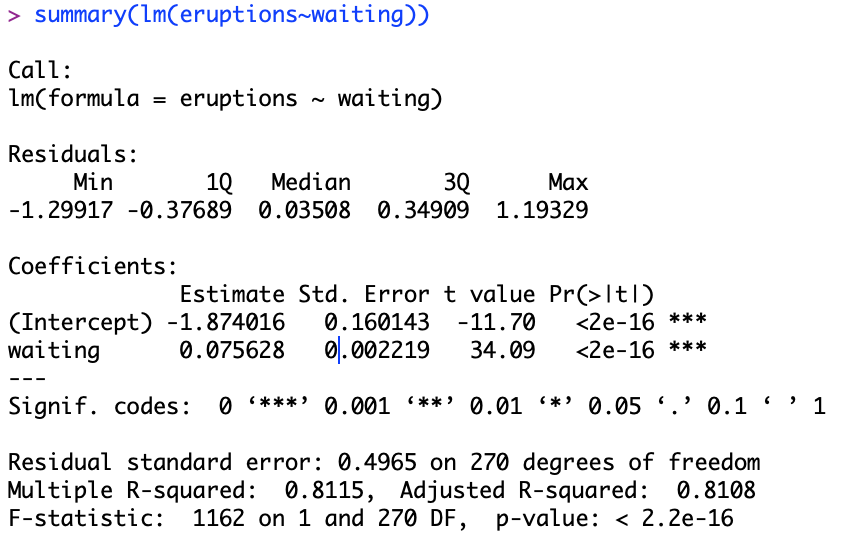
\includegraphics[width=3.5in]{images/geyserout.png}
    \end{center}
    Interpret the $R^2$ value for this model. \\What else can we learn from the \texttt{R} output?
\end{frame}

\begin{frame}{Regression Example}
    \vspace{-18pt}\begin{center}
        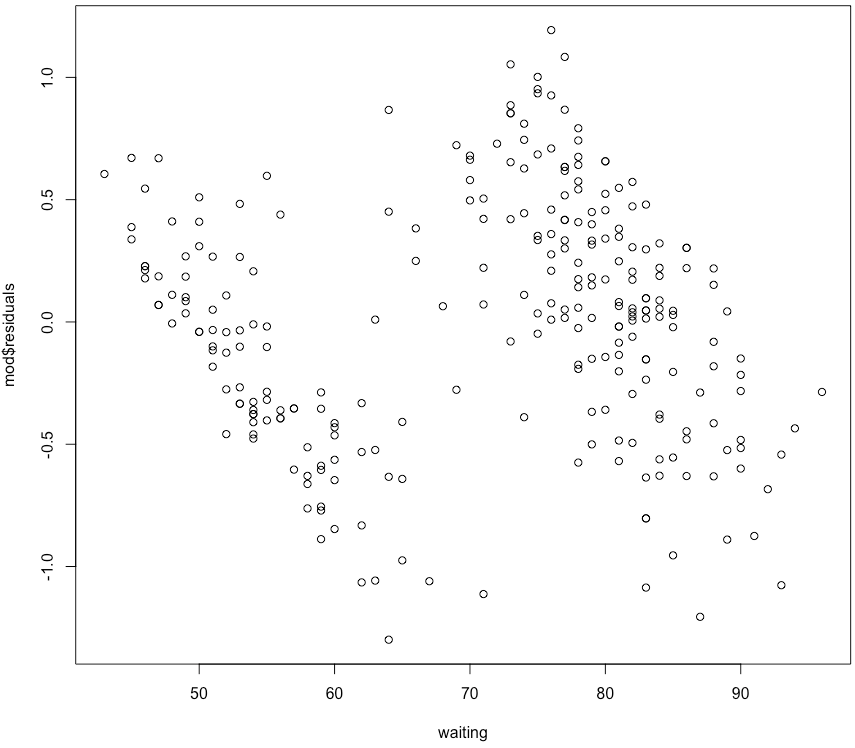
\includegraphics[scale=0.25]{images/geyserResid.png}
    \end{center}
    \vspace{-12pt}This is the residual plot for the geyser regression. Do you see any problems?
\end{frame}

\begin{frame}{Regression Example}
    \vspace{-18pt}\begin{center}
        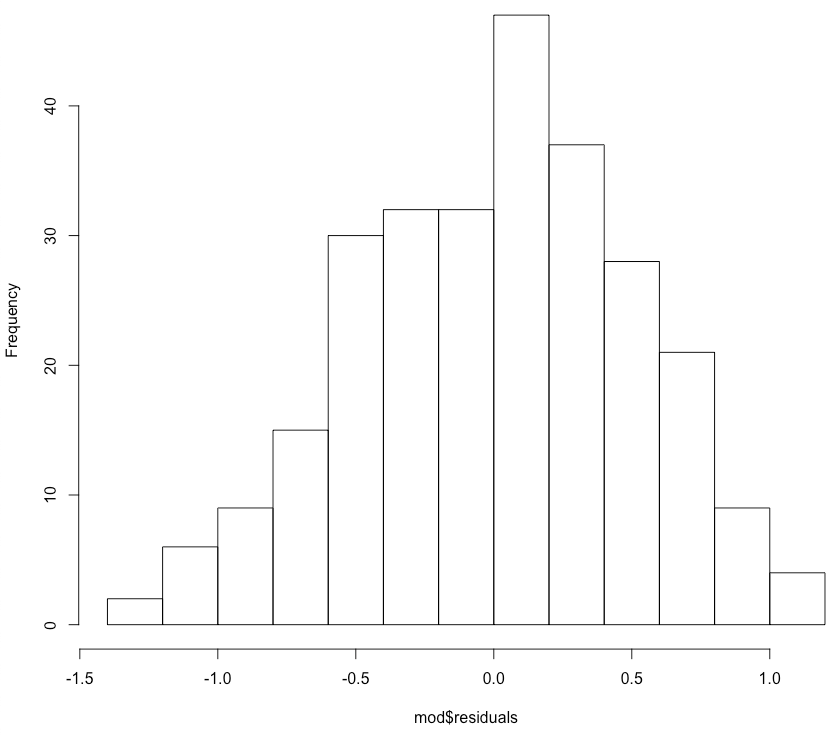
\includegraphics[scale=0.25]{images/residhist.png}
    \end{center}
    \vspace{-12pt}This is a histogram of the residuals. Do they look normally distributed?
\end{frame}

\begin{frame}{More Regression Diagnostics}
    \vspace{-0.5cm}\begin{center}
        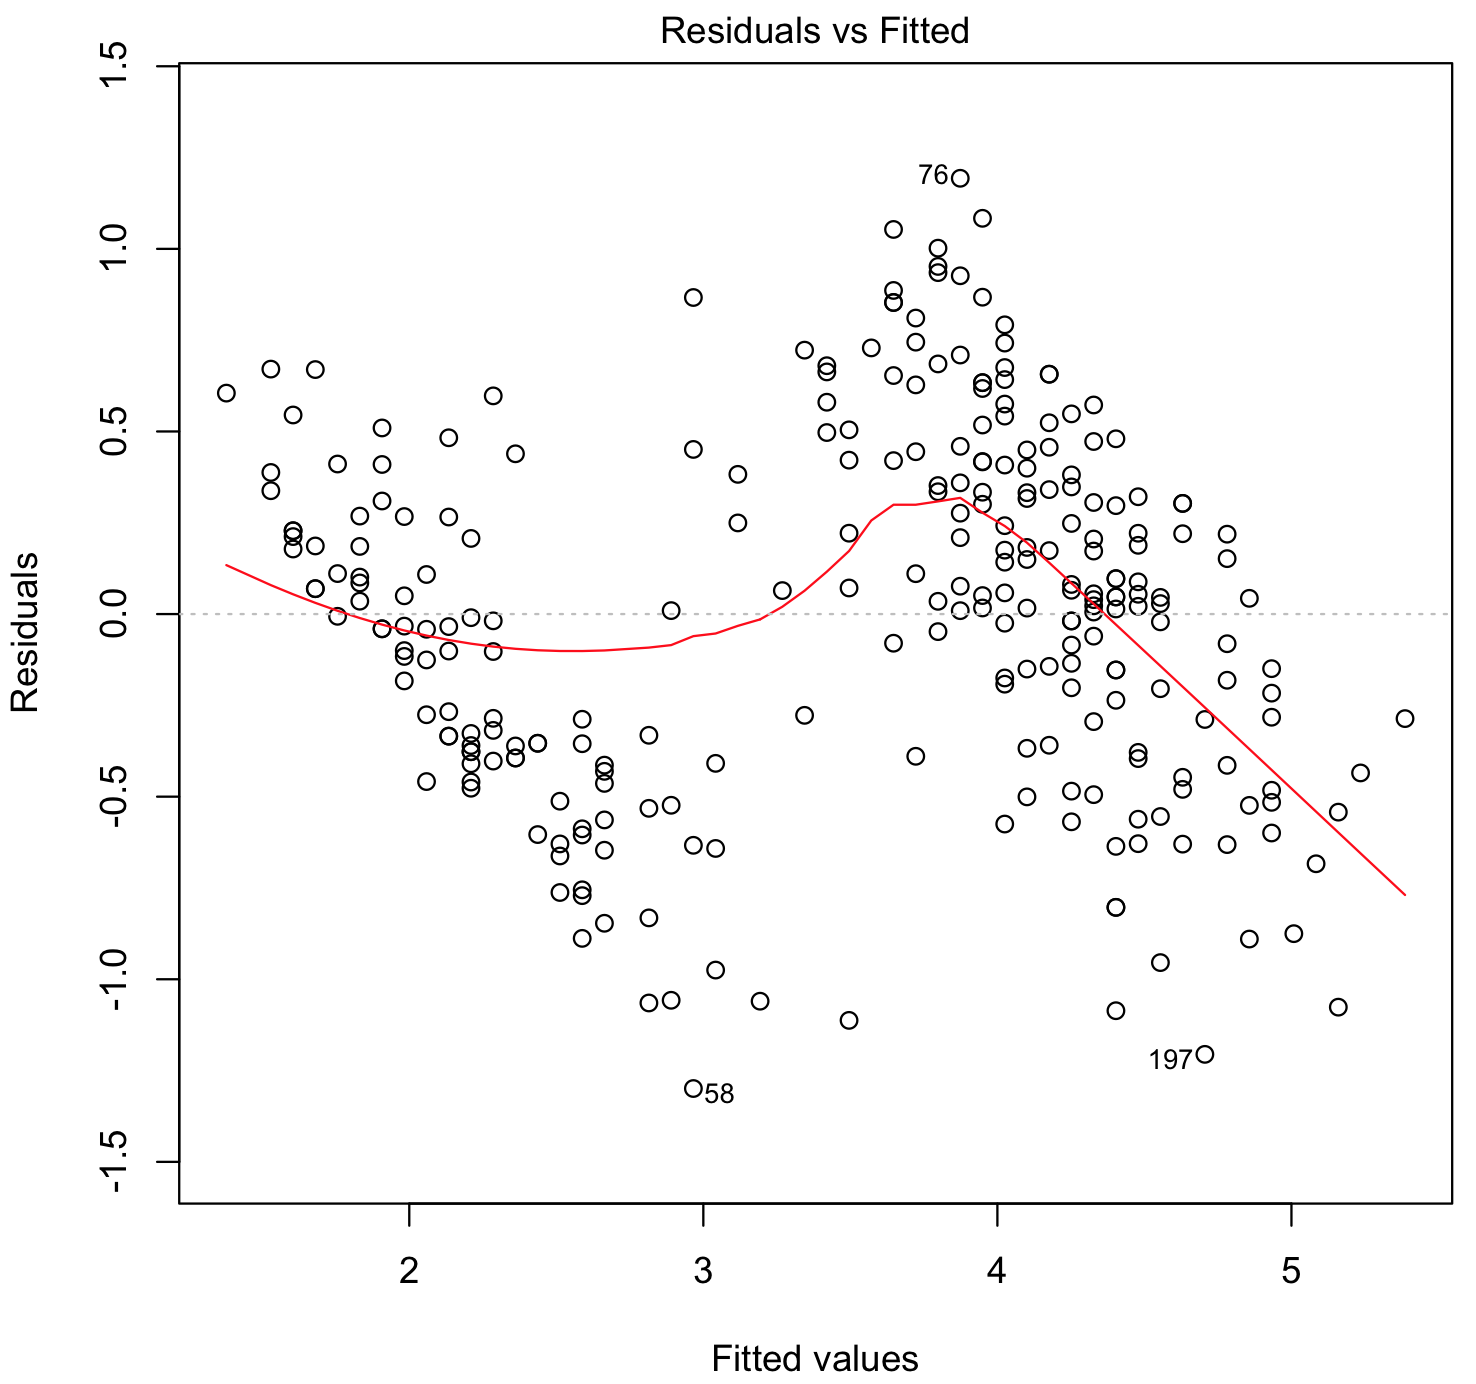
\includegraphics[height=2.5in]{images/residfaith.png}
    \end{center}
    Residuals vs. fitted values in R for the \texttt{faithful} data.
    % R model plot output: Residuals vs fitted values (R gives extra info)
\end{frame}

\begin{frame}{The Normal Q-Q Plot}
    \vspace{-0.5cm}\begin{center}
        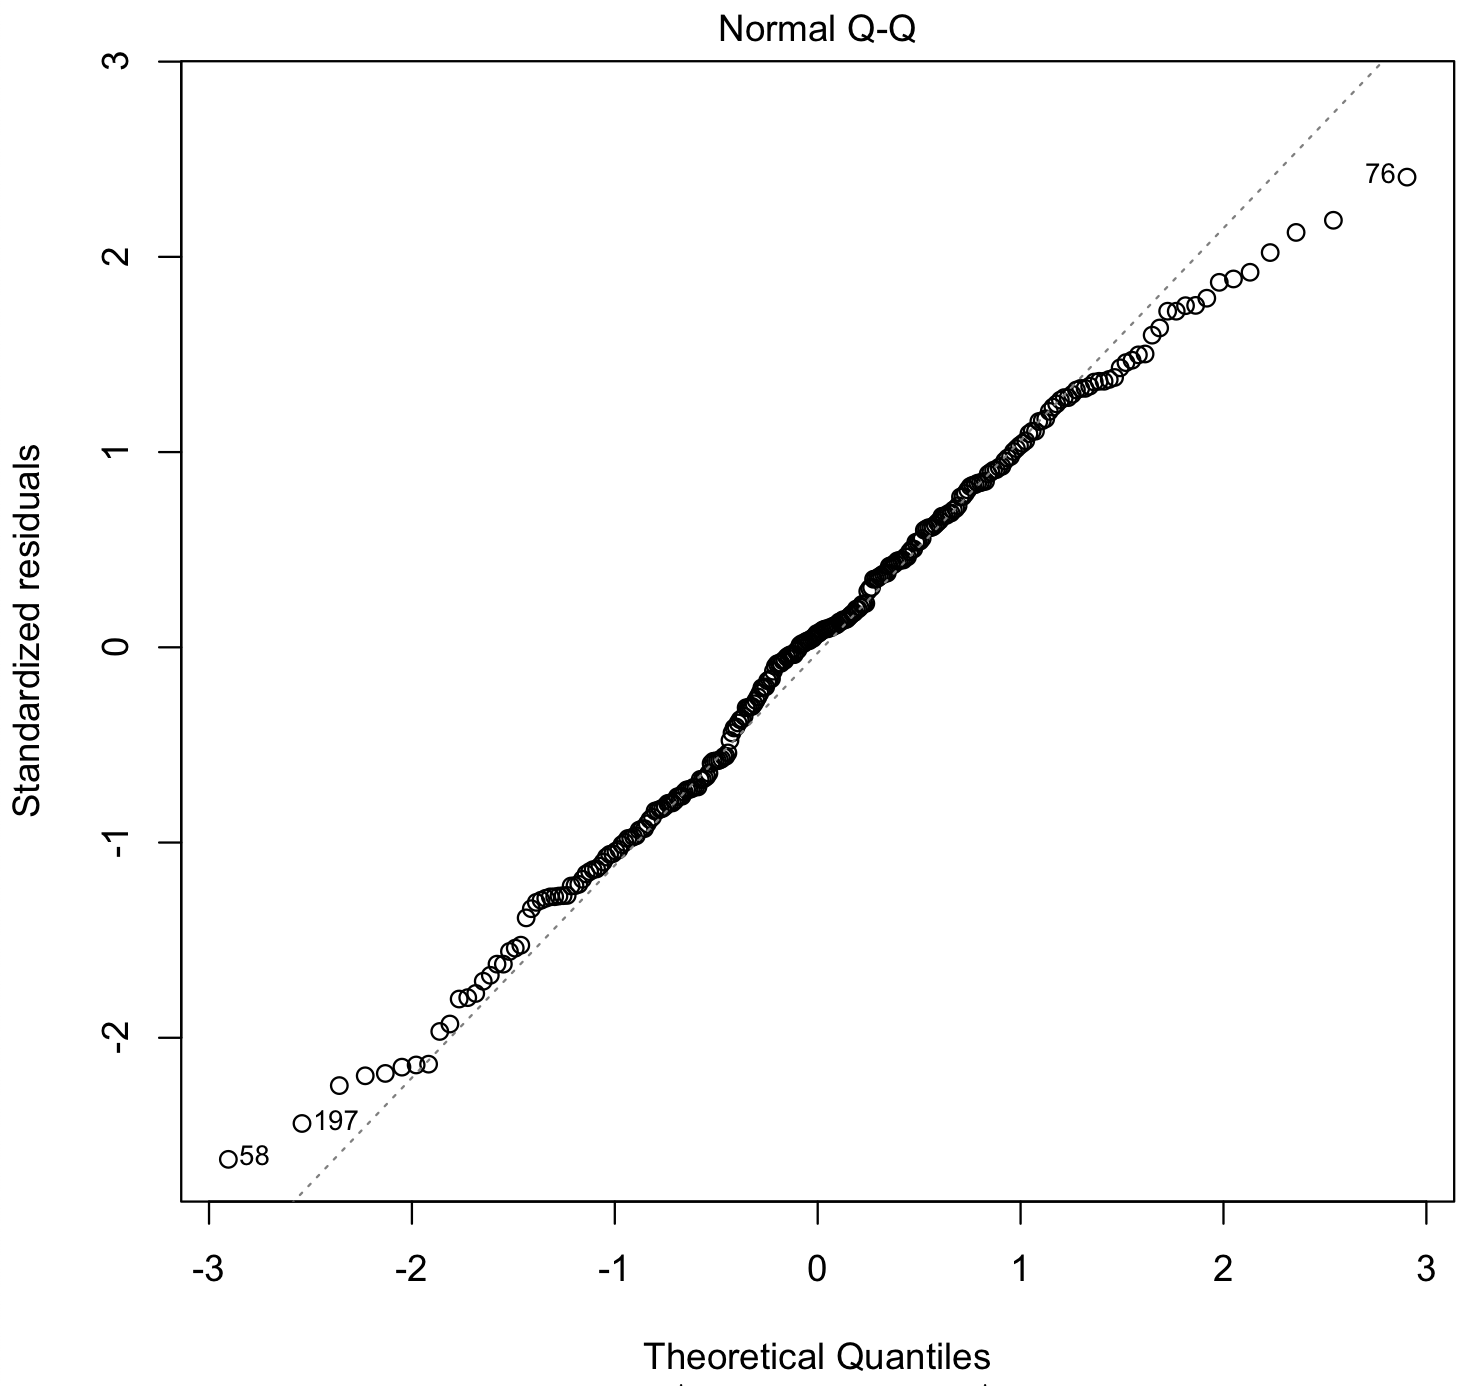
\includegraphics[height=2.5in]{images/qqplot.png}
    \end{center}
    The normal quantile-quantile (QQ) plot for the \texttt{faithful} data.
    % Normal Q Q plots
\end{frame}

\begin{frame}{The Scale-Location Plot}
    \vspace{-0.5cm}\begin{center}
        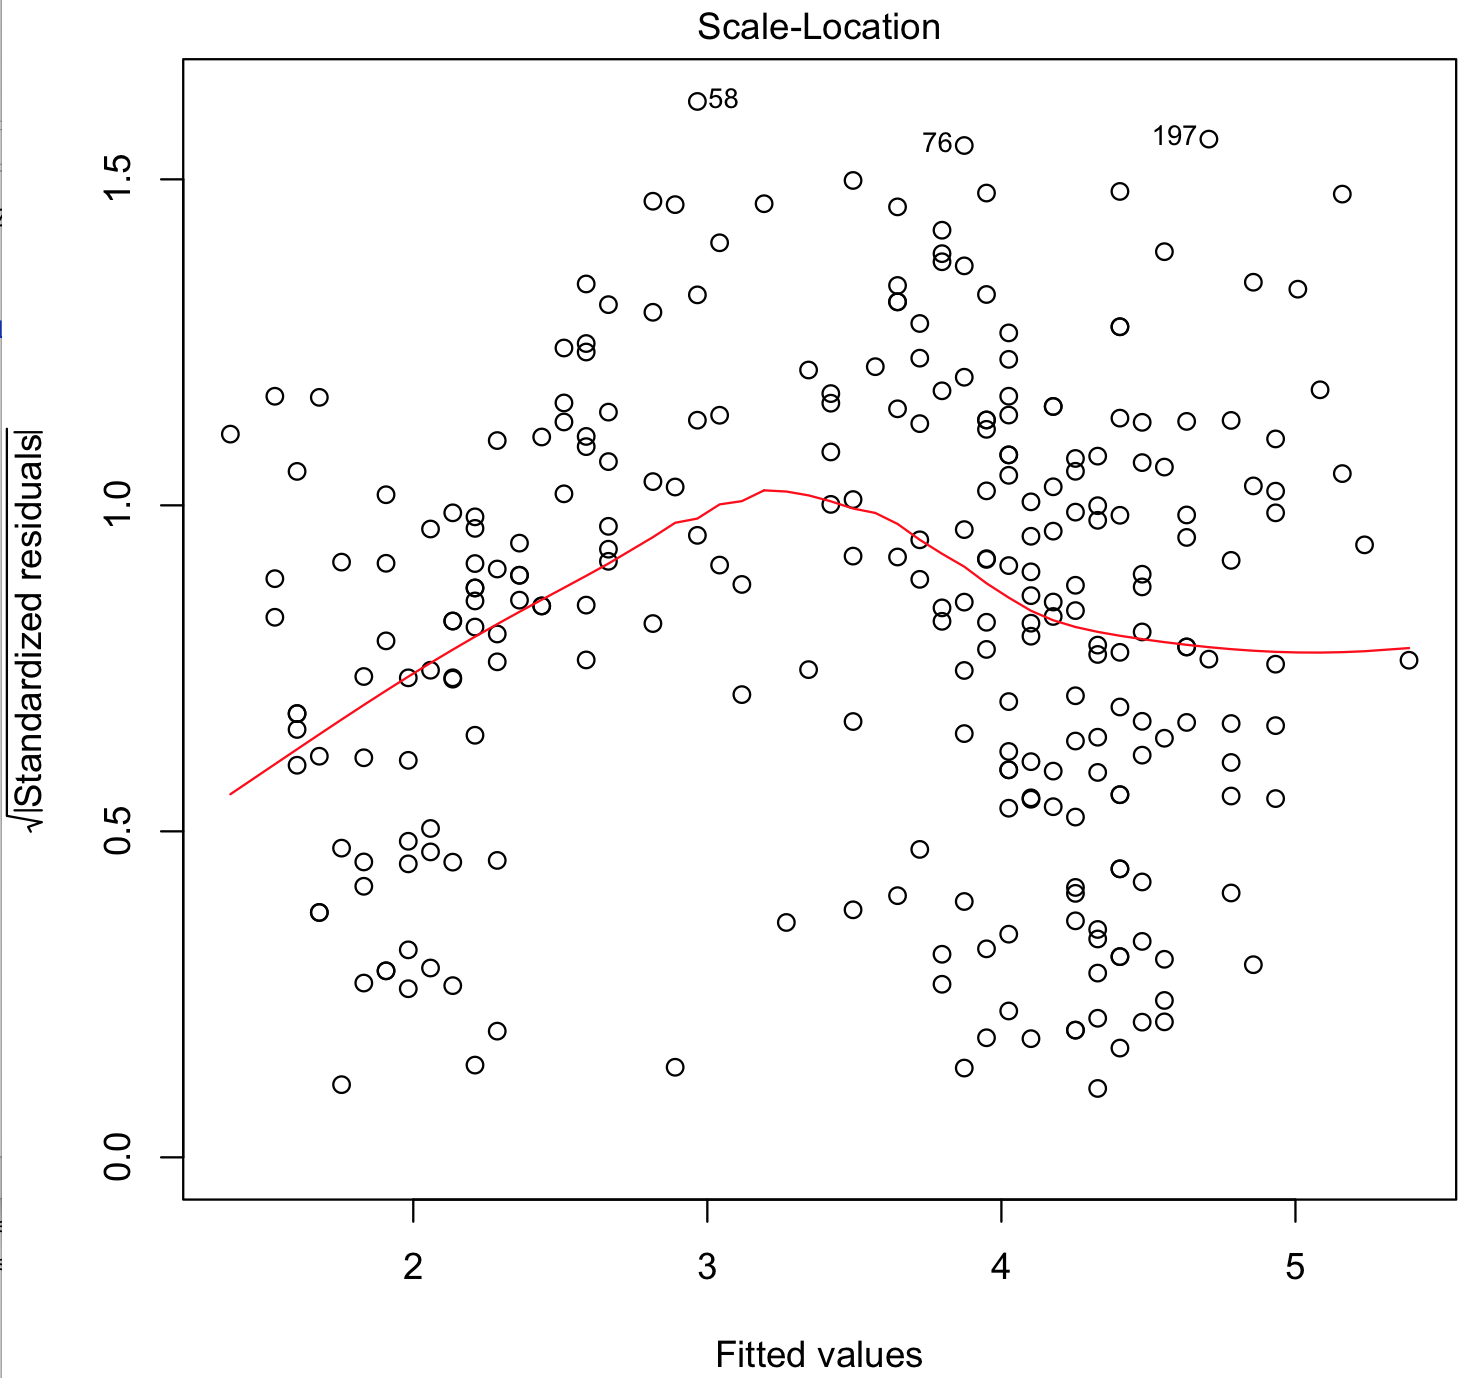
\includegraphics[height=2.5in]{images/scaleloc.png}
    \end{center}
    The scale-location plot for the \texttt{faithful} data.
    % Scale location (just mention that it's another way to look for constant variance)
\end{frame}

\begin{frame}{Categorical Predictors with Two Levels}
    \begin{itemize}
        \item We can also use categorical variables to predict outcomes!
        \item Under our current set up, we can use a categorical predictor with two levels.
        \item Later:
        \begin{itemize}
            \item We will examine predictors with multiple levels.
            \item We will examine response variables with two levels.
        \end{itemize}
    \end{itemize}
\end{frame}

\begin{frame}{Example}
    \hspace{1.5cm}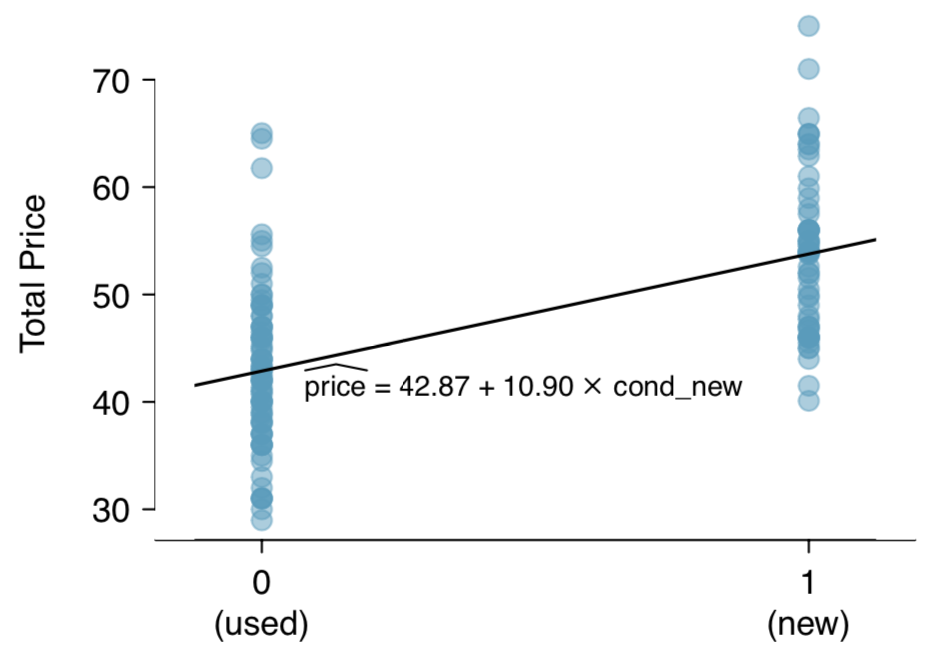
\includegraphics[width=3in]{images/binarypredictor.png}
    \begin{itemize}
        \item Consider Ebay auctions for Mario Kart Wii.
        \item We want to know how game \texttt{condition} affects selling \texttt{price}.
    \end{itemize}
\end{frame}

\begin{frame}{Example}
    To use \texttt{condition} in a regression, we use a \textbf{indicator variable}.
    \begin{itemize}
        \item An indicator variable always takes the values 0 or 1.
        \item Let $x=0$ when \texttt{condition} is \texttt{used}. 
        \item Let $x=1$ when \texttt{condition} is \texttt{new}. 
        \item We are \textit{indicating} whether the game is new. 
    \end{itemize}
\end{frame}

\begin{frame}{Example}
    Using our indicator variable for \texttt{condition},
    \begin{align*}
        \hat{\text{price}} &= b_0 + b_1 x \\
                        &= 42.87 + 10.90 x
    \end{align*}
    Interpret the model parameters. 
\end{frame}
